\appendix
\chapter{Full Application Examples}

The following sections provide a demonstration of working code using the current MELON library implementation in JRuby.

\section{News Server \& Reader Applications}

\begin{lstlisting}[caption={News Reader}, label={code:newsserverfull}]
require "melon"

# Initialize MELON
melon = Melon.with_zmq

# Initialize potential topics
topics = ["Politics", "Sports", "Business", "Technology", "Local"]

i = 0

loop do
  # Choose a topic
  topic = topics.sample
  
  # Generate headline for topic
  message = [topic, "#{topic} news item #{i+=1}"]
  
  # Write message
  melon.write message
  
  # Pause for a few seconds
  sleep rand(5)
end
\end{lstlisting}


\begin{lstlisting}[caption={News Reader}, label={code:newsreaderfull}]
require "melon"

unless ARGV[2]
  abort "news_reader.rb ADDRESS PORT TOPIC"
end

address = ARGV[0]
port = ARGV[1]
topic = ARGV[2]

# Initialize MELON
melon = Melon.with_zmq

# Add address of a news server
melon.add_remote port, address

# Set the template to retrieve a headline for the
# given topic
template = [topic, String]

# Read all relevant messages as they become available
loop do
  puts melon.read_all template
end
\end{lstlisting}

\section{Chat Application}

This example splits the implementation of a chat application into a library which provides most of the functionality and a small script to set up the environment for the user.

\begin{lstlisting}[caption={Chat Library}, label={code:chatlibfull}]
# Encapsulate chat communication
class Chat
  def initialize name
    @name = name
    @melon = Melon.with_zmq
  end

  def add_remote port
    @melon.add_remote port
  end
  
  # Write out a chat message
  def chat message
    @melon.write [@name, message]
  end

  # Get all unseen messages
  def read_messages
    @melon.read_all [String, String]
  end
 
  # Print out all messages except our own  
  def print_messages messages
    messages.each do |name, message|
      unless name == @name
        puts "\n<#{name}> #{message}"
      end
    end
  end

  # Read and show messages in a separate thread
  def monitor
    Thread.new do
      loop do
        print_messages read_messages
      end
    end
  end

  # Main loop for chatting
  def start
    monitor

    # Send chat messages from user
    loop do
      print "? "
      message = gets.strip

      unless message.empty?
        chat message
      end
    end
  end
end
\end{lstlisting}

The chat client in Listing \ref{code:chatclientfull} is a simple script to set up a chat client that talks to other local chat clients. This makes it simple to try on a single machine.

\begin{lstlisting}[caption={Local Chat Client}, label={code:chatclientfull}]
require "melon"
require "chat"

# Get user's name
print "Name: "
name = gets.strip

# Initialize chat library
chat = Chat.new name

# Add processes running on the same machine but different ports
loop do
  print "Remote port: "
  chat.add_remote gets.strip.to_i

  print "Add another (y/n)? "
  break unless gets.downcase.start_with? "y"
end

# Start chatting
chat.start
\end{lstlisting}

\chapter{MELON Prototype Implementation Details}

This appendix describes the prototype implementation of MELON in more detail.

\section{Local Storage}

Each application manages its own local storage, implemented as the \texttt{LocalStorage} class. Each instance of \texttt{LocalStorage} consists of two dynamic arrays: one for read-only messages and one for take-only messages. The class provides methods for storing, retrieving, and reading messages from these arrays.

\begin{table}\footnotesize
\centering
\caption{LocalStorage Methods}
\begin{tabular}{|c|c|c|p{5cm}|} \hline
\textbf{Method} & \textbf{Input} & \textbf{Output} & \textbf{Description} \\ \hline
store & message & & Stores a take-only message \\ \hline
write & message & & Stores a read-only message \\ \hline
find\_and\_take & template & message & Removes matching take-only message \\ \hline
take\_all & template & messages & Removes all matching take-only messages  \\ \hline
find\_unread & template, read\_messages & message & Returns matching read-only message  \\ \hline
find\_all\_unread & template, read\_messages & messages & Returns all matching read-only messages  \\ \hline
\end{tabular}
\label{fig:localstorageimpl}
\end{table}

When a new message is added to the store a new \texttt{StoredMessage} object is created. The local storage generates a incremental ID for the new \texttt{StoredMessage}. Once it obtains an exclusive lock for the appropriate array, the message is added to the end of the array.

Retrieving a take-only message involves scanning the take-only array for a matching message. If one is found, the scan stops. The matching message is deleted from the array and the message is returned. If not matching message is found, the method returns \texttt{nil}. When scanning, the mutex associated with the take-only array is locked.

Finding a read-only message is a little more involved because the local storage must avoid returning any messages which have already been read. As it scans, it only attempts matching messages which are not included in the provided \texttt{read\_messages} data structure. Unlike the take-only removal, many reads may occur at the same time. For this reason, a readers/writers lock is used for accessing the read-only array. This allows multiple readers but only a single writer to access the array.

Bulk operations are essentially the same, except all matching messages are returned instead of just the first matching.

\subsection{Messages}

In the prototype, messages are arrays which may contain any assortment of values. Templates are also arrays, but if a value is a class it will be matched against the class of the value in the message. Please note MELON may be implemented with any message scheme that allows for matching based on some kind of templates, this was just a simple approach used in the prototype implementation.

\subsection{Stored Messages}

When a message is stored, it is saved in a \texttt{StoredMessage} which holds an ID and a \textit{copy} of the message. This prevents issues if the message is modified after being stored.

The \texttt{StoredMessage} class implements a simple message matching algorithm. First, if the message is not the same length as the template, clearly they do not match. Otherwise, the template and the message are compared value by value. If the template value is a class, the message value is checked to see if it is an object of the same class or a subclass. Otherwise, the values are compared via equality. The matching aborts on the first mismatch.

\texttt{StoredMessage} also implements the mapping of process ID and message ID to a single integer as described in Equation \ref{eq:elegantpairing}, resulting in the identifier used for tracking the message in the read message data structures.

\section{Remote Storage Client}

All network communication in the prototype is implemented using ZeroMQ.

Each remote storage client, implemented in the \texttt{RemoteStorage} class, is associated with a particular remote node specified by an IP address and port. \texttt{RemoteStorage} offers exactly the same retrieval API as local storage, so the MELON API implementation may treat local storage and remote storage in the same manner.

When a method is called on a \texttt{RemoteStorage}, it serializes the method name, template, and read messages (if a read-only action) and sends them to the remote node. If the remote node is unavailable, the communication times out and the method returns \texttt{nil}. Choosing a timeout value presents a trade-off. Lower values allow operations to return faster if the remote node is unavailable, but then the communication is less reliable. Higher values are slower, but may provide greater opportunities for connections. In our implementation we allowed 1.5 seconds for sending to the remote node and 5 seconds for receiving the reply.

When a response is received, it is deserialized and returned to the caller.

\section{Remote Storage Server}

The storage server as implemented in the \texttt{StorageServer} class, is the most complicated piece of the prototype because it must manage multiple concurrent connections. To do so, it manages a thread pool of workers to accept connections. As remote nodes connect, the connections are handed to the workers over an interprocess connection using ZeroMQ. The worker then deserializes the message and calls the appropriate method on the local storage. Assuming the message is valid, the result from the local storage is again serialized and returned to the remote node.

In the implementation, the server provides a ZeroMQ ``ROUTER'' socket to which the remote nodes connect using a ``REQ'' socket. Internally, the server provides a ``DEALER'' socket which each of the workers connects to via a ``REP'' sockets. Then the sever connects the ``ROUTER'' socket to the ``DEALER'' via a queue. This allows multiple incoming requests to be handed off to the workers. Figure \ref{fig:zeromqserver} shows the relationship between the different components.

\begin{figure}
\centering
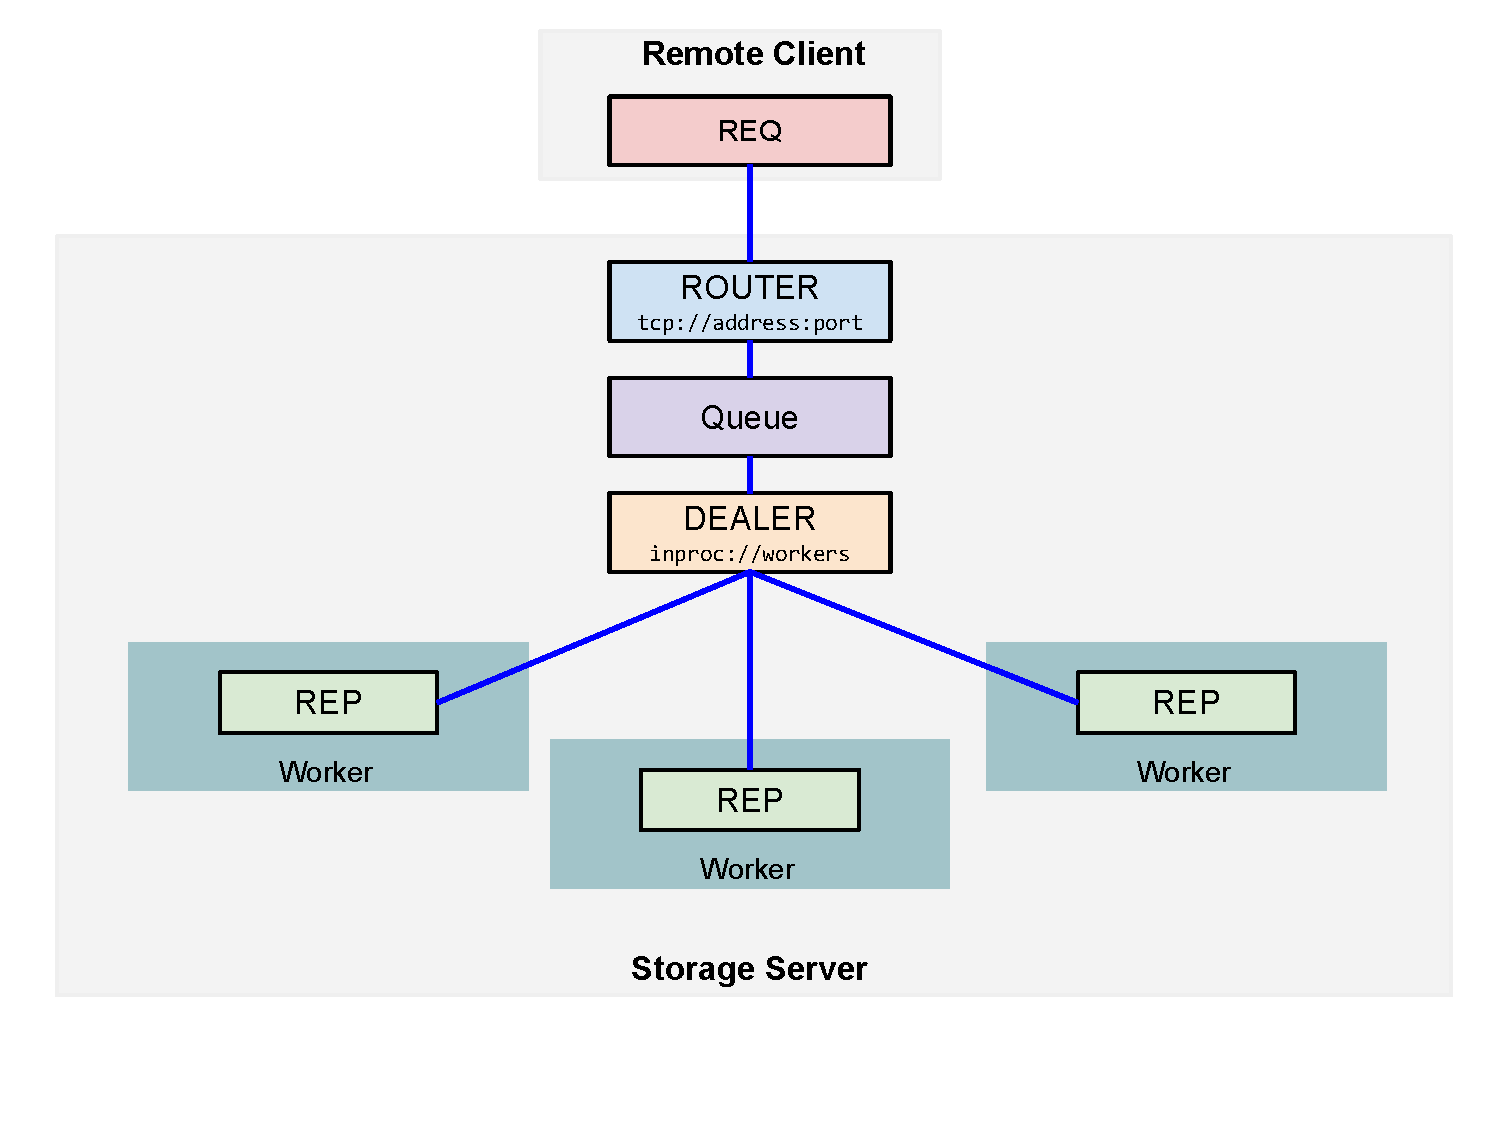
\includegraphics[scale = .60, clip, trim = 0px 0px 0px 0px]{figures/zeromq-server.pdf}
\caption{ZeroMQ Server Setup}
\label{fig:zeromqserver}
\end{figure}

\section{MELON API}

The application developer only every needs to interact with the MELON API. The implementation of the API maintains a set of servers (local and remote storage) and the set of read messages. The API provides the six MELON operations and a method to add remote servers. The prototype implementation does not provide a mechanism for discovering remote nodes, so these must be added manually.

For \texttt{store}/\texttt{write}, the API saves the message directly to the local storage.

For the retrieval operations, the API iterates over the storage servers (local and remote) in a random order for each call, invoking the operation on each in turn. When retrieving a single message, the iteration aborts when a matching message is returned. In bulk operations, connections to all servers are attempted and the results returned in one array. If an operation is blocking and no messages are found, there is a brief delay (currently 1 second) then the iteration resumes. If the operation is non-blocking, the servers are only iterated through once. Again, for the prototype implementation remote servers are contacted one at a time, not multicasted.